
\documentclass[11pt]{article}
%\linespread{1.1}
\usepackage{graphicx,import}
\usepackage{amsmath}
\usepackage{setspace}
\usepackage{color}
\usepackage{float}
\usepackage[inkscapelatex=false,inkscapearea=page]{svg}
\onehalfspacing
%\doublespacing

\title {Architecture and Open Queue Formulas \\ \bigskip \large Thesis}
\date{21 September 2020}

\begin{document}
\maketitle
\section{Introduction}
This section will deal with the assumptions we've made so far and why we've made them. Alternatives will be described for the various possibilities.\\
\subsection{Assumptions}
\begin{enumerate}
\item \textbf{Assumption 1}: All layers have no horizontal connection. The scheme we will present in section 2 will feature LANs accessible by all nodes of the same layer so this type of communication is actually possible through those LANs, but for now decided to not have horizontality in the message system.
\item \textbf{Assumption 2}: The only entity needing a disk is the Central Node, in particular we are assuming that all other nodes receive information that can be processed, stored and aggregated in the RAM which will never be full. This is a strong assumption that can be relaxed if needed by adding disks in the regional and primary/secondary layer.
\item \textbf{Assumption 3}: The RAM element of the nodes doesn't need its own queue model, indeed it can be modeled in symbiosis with the CPU since it is used by only that component.
\item \textbf{Assumption 4}: In this first stage we won't be holding account of the fault tolerance of the system, in particular we are not considering duplication of the data not in storaging neither in multiple link sending.
\item \textbf{Assumption 5}:In the edge platform high level architecture document between a central node and the regionals there is a wan, and the same happens for the lower level. We propose two models, one having the wired WAN interpreted as a long distance LAN and another one where it is an actual WAN.
\end{enumerate}
\subsection{Table}
First of all, we started by compiling the table with the responses as we expect them to be. The green ones are those decisions we made while the black ones are trivial ones that have no alternatives.\\
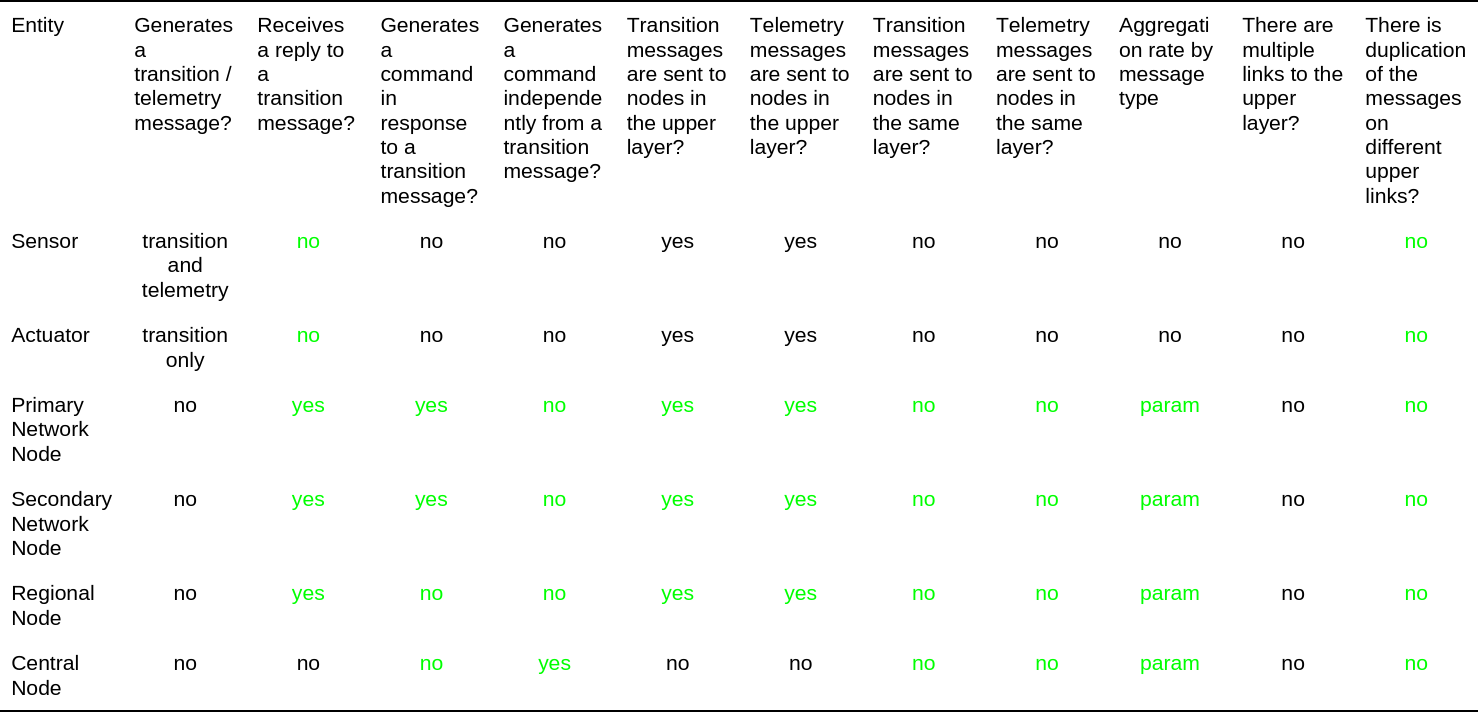
\includegraphics[width=15cm, height=10cm]{table.png}
Now, row by row we will justify or explain our answers:
\begin{enumerate}
\item Generate a transition or telemetry message: the sensor give telemetry informations to the upper node with a certain rate. Both actuators and sensor will generete a transitions message in the case that their state is changed without a transition command received. All others entities have no case in which they need to do so.
\item Receives a reply to a transition message: sensor and actuators don't need an acknowledgment from the upper level, while all other entities do. The only exception is the Central node since he doesn't have an upper node to send to.
\item Generates a command in response to a transition message: the primary reading the transition messages may need to issue commands to actuators in order to keep the system flowing.
\item Generates a command independently from a transition message: none of the entities may generate a command without any trigger, the only exception being the central node which sends commands when needed.
\item Transition messages are sent to nodes in the upper layer: all entities need to send to an upper level until the central node is reached.
\item Telemetry messages are sent to nodes in the upper layer: same as last one.
\item Transition messages are sent to nodes in the same layer: no, for assumption 1.
\item Telemetry messages are sent to nodes in the same layer: no, for assumption 1.
\item Aggregation rate by message type: we don't have the actual rate so we put a parameter in the aggregation formulas.
\item There are multiple links to the upper layer: not useful at the moment for modeling and queue formulas so we skipped over it. Also for Assumption 4 we may implement it in a later stage.
\item There is duplication of the messages on different upper links: No, for assumption 4.
\end{enumerate}

\section{Structural scheme}
First of all, due to assumption 5, the following is the extended LAN model:\\
\begin{figure}[H]
	\hspace*{-3.75cm}
	\centering
  \frame{\includesvg[width=20cm]{centralregional}}
  \caption{Focus on Central and Regional nodes}
\end{figure}
\begin{figure}[H]
	\hspace*{-3.75cm}
	\frame{\includesvg[width=20cm]{primarysecondary}}
	\caption{Focus on Regional and Primary/Secondary nodes}
\end{figure}
\begin{figure}[H]
	\hspace*{-3.75cm}
  \frame{\includesvg[width=20cm]{primarysensor}}
  \caption{Focus on Primary/Secondary nodes and end points}
\end{figure}
As it can be seen, between an upper level node and a lower level one there is a router connected to a LAN which receives and sends messages to all the lower level nodes. Keeping in mind assumption 1 on the horizontal level communication, even if the nodes on a level share a lan they can only send and receive from the upper level router.\\
Furthermore this iteration is parametric so a central node manages n regional nodes. Each regional node manages m primary and k secondary nodes, these parameters varies with the regional node they are associated to. Same thing extends to primary/secondary with respect to the sensors/actuators, respectively in numbers s and a.\\
One last note about the scheme is that at the moment we divided on two LANs primary and secondary for clarity since they have different rate, operations and technology. Likewise for the different communication technology with actuators and sensors.\\
The whole scheme:
\begin{figure}[H]
	\hspace*{-3.75cm}
	\frame{\includesvg[width=20cm]{structural_scheme_wan}}
  \caption{Structural scheme}
\end{figure}
\section{Queues Scheme}
\begin{figure}[H]
	\hspace*{-3.75cm}
	\frame{\includesvg[width=20cm]{queue_network_centralregional}}
	\caption{Focus on Central and Regional nodes}
\end{figure}
\begin{figure}[H]
	\hspace*{-3.75cm}
	\frame{\includesvg[width=20cm]{queue_network_primarysensor}}
	\caption{Focus on Regional nodes, Primary/Secondary nodes and sensor/actuators}
\end{figure}
\begin{figure}[H]
	\vspace*{-0.5cm}
	\hspace*{-3.75cm}
	\frame{\includesvg[width=20cm]{queue_network_wan}}
	\caption{The whole scheme}
\end{figure}

\section{Open Queues Formulas}

\section{Notation}
We will deline the notation in the following formulas, each of them has one or many subscripts for the item they refer to, the same type of element in a different part has the same notation even though it's not the same element:
\begin{itemize}
\item $\lambda_t$ and $\lambda_e$: $\lambda$ is the arrival rate, respectively for the data type telemetry and transition.
\item $V$: mean number of visits.
\item $S$: service time.
\item $D$: service demand.
\item $U$: utilization factor.
\item $R$: response time.
\end{itemize}

The various elements are called:
\begin{itemize}
\item Lan: $l$;
\item CPU: $c$;
\item Disk: $d$.
\end{itemize}
Each node has a summary section which describes the total response time for that node type.\\
To develop the following formulas, we started from the network queue in the case of an open network.

\section{Node}


%\begin{itemize}
%
%    \item $\lambda_t$, arrival rate for telemetry data
%    \item $\lambda_e$, arrival rate for events data
%    \item $S_{node\_wlan, \ t}$, service time wifi lan
%    \item $V_{node\_wlan, \ t}$, number of visits to wifi lan
%    \item $S_{node\_wlan, \ e}$, service time wifi lan
%    \item $V_{node\_wlan, \ e}$, number of visits to wifi lan
%
%    \item $S_{node\_cpu, \ t}$, service time wifi lan
%    \item $V_{node\_cpu, \ t}$, number of visits to wifi lan
%    \item $S_{node\_cpu, \ e}$, service time wifi lan
%    \item $V_{node\_cpu, \ e}$, number of visits to wifi lan
%
%    \item $S_{node\_ram, \ t}$, service time wifi lan
%    \item $V_{node\_ram, \ t}$, number of visits to wifi lan
%    \item $S_{node\_ram, \ e}$, service time wifi lan
%    \item $V_{node\_ram, \ e}$, number of visits to wifi lan
%
%    \item $S_{node\_lan, \ t}$, service time wifi lan
%    \item $V_{node\_lan, \ t}$, number of visits to wifi lan
%    \item $S_{node\_lan, \ e}$, service time wifi lan
%    \item $V_{node\_lan, \ e}$, number of visits to wifi lan
%
%\end{itemize}



\subsection{Wifi card}
In the equations of the wifi card, the element is called $w$. So $V_{w, t}$ is the mean number of visits for the wifi card in the case of a telemetry data type.\\
For the wifi card, since there are 4 sensors, the arrival rate for the telemetry data type is four times the total arrival rate, while due to the single actuator, in the case of a transition event the arrival rate is exactly the same.
\begin{equation}
    \begin{array}{l}
        V_{w, t} = 1 \\
        V_{w, e} = 1 \\
        \lambda_{w, t} = 4*\lambda_{t} \\ %4 sensors
        \lambda_{w, e} = \lambda_{e} \\ %1 actuator
    \end{array}
\end{equation}

\begin{equation}
    \begin{array}{l}
        D_{w, t} = V_{w, t} * S_{w, t} \\
        D_{w, e} = V_{w, e} * S_{w, e} \\
        U_{w, t} = \lambda_{w, t} * D_{w, t} \\
        U_{w, e} = \lambda_{w, e} * D_{w, e} \\
        U_{w} = U_{w, t} + U_{w, e} \\
        R_{w, t} = \frac{D_{w, t}}{1 - U_{w}} \\
        R_{w, e} = \frac{D_{w, e}}{1 - U_{w}} \\
    \end{array}
\end{equation}

\subsection{Ram}
The mean number of visits for the transition events is two because after receiving it you need to reply and thus the visits double.
\begin{equation}
    \begin{array}{l}
        V_{r, t} = 1 \\
        V_{r, e} = 2 \\ %reply
        \lambda_{r, t} = \lambda_{w, t} \\
        \lambda_{r, e} = \lambda_{w, e} \\
    \end{array}
\end{equation}

\begin{equation}
    \begin{array}{l}
        D_{r, t} = V_{r, t} * S_{r, t} \\
        D_{r, e} = V_{r, e} * S_{r, e} \\
        U_{r, t} = \lambda_{r, t} * D_{r, t} \\
        U_{r, e} = \lambda_{r, e} * D_{r, e} \\
        U_{r} = U_{r, t} + U_{r, e} \\
        R_{r, t} = \frac{D_{r, t}}{1 - U_{r}} \\
        R_{r, e} = \frac{D_{r, e}}{1 - U_{r}} \\
    \end{array}
\end{equation}

\subsection{Lan}
As in the ram, since there is a reply needed for the transition type the mean number of visits doubles.
Every two received messages of the telemetry type, we aggregate them in a single message and send them to the upper level, thus the halving of the arrival rate.
\begin{equation}
    \begin{array}{l}
        V_{l, t} = 1 \\
        V_{l, e} = 2 \\ %reply
        \lambda_{l, t} = \frac{\lambda_{w, t}}{2} \\ %ogni 2 msg ricevuti, aggreghi e invii
        \lambda_{l, e} = \lambda_{w, e} \\
    \end{array}
\end{equation}

\begin{equation}
    \begin{array}{l}
        D_{l, t} = V_{l, t} * S_{l, t} \\
        D_{l, e} = V_{l, e} * S_{l, e} \\
        U_{l, t} = \lambda_{l, t} * D_{l, t} \\
        U_{l, e} = \lambda_{l, e} * D_{l, e} \\
        U_{l} = U_{l, t} + U_{l, e} \\
        R_{l, t} = \frac{D_{l, t}}{1 - U_{l}} \\
        R_{l, e} = \frac{D_{l, e}}{1 - U_{l}} \\
    \end{array}
\end{equation}

\subsection{Cpu}
We will now make a note that will be useful for following formulas as well, focusing on the service demand in both data type cases.\\
\begin{itemize}
\item $\frac{1}{2}S_{c, t, mem} + \frac{1}{2}S_{c, t, aggr}$ : in the cpu service demand for the telemetry case, we put the sum of half the service time in memorization and aggregation because the aggregation rate is $\frac{1}{2}$. Indeed, each time a telemetry event arrives can trigger one of the two actions with the same probability.
\item $\frac{1}{2}S_{c, e, new} + \frac{1}{2}S_{c, e, repl}$ : specularly in the case of a transition event, the two cases are when the cpu receives a new message or it receives an acknowledgment of a message it already sent.
\end{itemize}

\begin{equation}
    \begin{array}{l}
        V_{c, t} = 1 \\
        V_{c, e} = 2 \\ %reply
        \lambda_{c, t} = \lambda_{w, t} \\
        \lambda_{c, e} = \lambda_{w, t} \\
    \end{array}
\end{equation}

\begin{equation}
    \begin{array}{l}
        D_{c, t} = V_{c, t} * (\frac{1}{2}S_{c, t, mem} + \frac{1}{2}S_{c, t, aggr}) \\ %(1 - 1/aggregazione)
        D_{c, e} = V_{c, e} * (\frac{1}{2}S_{c, e, new} + \frac{1}{2}S_{c, e, repl}) \\
        U_{c, t} = \lambda_{c, t} * D_{c, t} \\
        U_{c, e} = \lambda_{c, e} * D_{c, e} \\
        U_{c} = U_{c, t} + U_{c, e} \\
        R_{c, t} = \frac{D_{c, t}}{1 - U_{c}} \\
        R_{c, e} = \frac{D_{c, e}}{1 - U_{c}} \\
    \end{array}
\end{equation}

\subsection{Summary}
\begin{equation}
    \begin{array}{l}
        R_{node, \ t} = R_{w, t} + R_{r, t} + R_{c, t} + R_{l, t} \\
        R_{node, \ e} = R_{w, e} + R_{r, e} + R_{c, e} + R_{l, e} \\
    \end{array}
\end{equation}


\section{Regional Node}

\subsection{Lan down}
The arrival rate for transition type formula is given by the fact that there are two clients but there is aggregation so we have $\frac{\lambda_{w, t}}{2}$ for each client.
\begin{equation}
    \begin{array}{l}
        V_{ld, t} = 1 \\
        V_{ld, e} = 2 \\
        \lambda_{ld, t} = 2*\frac{\lambda_{w, t}}{2} \\ %two client but aggregation
        \lambda_{ld, e} = 2*\lambda_{w, e} \\
    \end{array}
\end{equation}

\begin{equation}
    \begin{array}{l}
        D_{ld, t} = V_{ld, t} * S_{ld, t} \\
        D_{ld, e} = V_{ld, e} * S_{ld, e} \\
        U_{ld, t} = \lambda_{ld, t} * D_{ld, t} \\
        U_{ld, e} = \lambda_{ld, e} * D_{ld, e} \\
        U_{ld} = U_{ld, t} + U_{ld, e} \\
        R_{ld, t} = \frac{D_{ld, t}}{1 - U_{ld}} \\
        R_{ld, e} = \frac{D_{ld, e}}{1 - U_{ld}} \\
    \end{array}
\end{equation}

\subsection{Ram}

\begin{equation}
    \begin{array}{l}
        V_{r, t} = 1 \\
        V_{r, e} = 2 \\ %reply
        \lambda_{r, t} = \lambda_{ld, t} \\
        \lambda_{r, e} = \lambda_{ld, e} \\
    \end{array}
\end{equation}

\begin{equation}
    \begin{array}{l}
        D_{r, t} = V_{r, t} * S_{r, t} \\
        D_{r, e} = V_{r, e} * S_{r, e} \\
        U_{r, t} = \lambda_{r, t} * D_{r, t} \\
        U_{r, e} = \lambda_{r, e} * D_{r, e} \\
        U_{r} = U_{r, t} + U_{r, e} \\
        R_{r, t} = \frac{D_{r, t}}{1 - U_{r}} \\
        R_{r, e} = \frac{D_{r, e}}{1 - U_{r}} \\
    \end{array}
\end{equation}

\subsection{Lan Up}

\begin{equation}
    \begin{array}{l}
        V_{lu, t} = 1 \\
        V_{lu, e} = 2 \\ %replay
        \lambda_{lu, t} = \frac{\lambda_{ld, t}}{2} \\ %ogni 2 msg ricevuti, aggreghi e invii
        \lambda_{lu, e} = \lambda_{ld, e} \\
    \end{array}
\end{equation}

\begin{equation}
    \begin{array}{l}
        D_{lu, t} = V_{lu, t} * S_{lu, t} \\
        D_{lu, e} = V_{lu, e} * S_{lu, e} \\
        U_{lu, t} = \lambda_{lu, t} * D_{lu, t} \\
        U_{lu, e} = \lambda_{lu, e} * D_{lu, e} \\
        U_{lu} = U_{lu, t} + U_{lu, e} \\
        R_{lu, t} = \frac{D_{lu, t}}{1 - U_{lu}} \\
        R_{lu, e} = \frac{D_{lu, e}}{1 - U_{lu}} \\
    \end{array}
\end{equation}

\subsection{Cpu}

\begin{equation}
    \begin{array}{l}
        V_{c, t} = 1 \\
        V_{c, e} = 2 \\ %replay
        \lambda_{c, t} = \lambda_{ld, t} \\
        \lambda_{c, e} = \lambda_{ld, e} \\
    \end{array}
\end{equation}

\begin{equation}
    \begin{array}{l}
        D_{c, t} = V_{c, t} * (\frac{1}{2}S_{c, t, mem} + \frac{1}{2}S_{c, t, aggr}) \\ %(1 - 1/aggregazione)
        D_{c, e} = V_{c, e} * (\frac{1}{2}S_{c, e, new} + \frac{1}{2}S_{c, e, repl}) \\
        U_{c, t} = \lambda_{c, t} * D_{c, t} \\
        U_{c, e} = \lambda_{c, e} * D_{c, e} \\
        U_{c} = U_{c, t} + U_{c, e} \\
        R_{c, t} = \frac{D_{c, t}}{1 - U_{c}} \\
        R_{c, e} = \frac{D_{c, e}}{1 - U_{c}} \\
    \end{array}
\end{equation}


\subsection{Summary}
\begin{equation}
    \begin{array}{l}
        R_{regional, \ t} = R_{ld, t} + R_{r, t} + R_{c, t} + R_{lu, t} \\
        R_{regional, \ e} = R_{ld, e} + R_{r, e} + R_{c, e} + R_{lu, e} \\
    \end{array}
\end{equation}

\section{Central}


\subsection{Lan}

\begin{equation}
    \begin{array}{l}
        V_{l, t} = 1 \\
        V_{l, e} = 2 \\ %reply
        \lambda_{l, t} = 2*\frac{\lambda_{ld, t}}{2} \\ %ogni 2 msg ricevuti, aggreghi e invii
        \lambda_{l, e} = 2*\lambda_{ld, e} \\
    \end{array}
\end{equation}

\begin{equation}
    \begin{array}{l}
        D_{l, t} = V_{l, t} * S_{l, t} \\
        D_{l, e} = V_{l, e} * S_{l, e} \\
        U_{l, t} = \lambda_{l, t} * D_{l, t} \\
        U_{l, e} = \lambda_{l, e} * D_{l, e} \\
        U_{l} = U_{l, t} + U_{l, e} \\
        R_{l, t} = \frac{D_{l, t}}{1 - U_{l}} \\
        R_{l, e} = \frac{D_{l, e}}{1 - U_{l}} \\
    \end{array}
\end{equation}

\subsection{Ram}

\begin{equation}
    \begin{array}{l}
        V_{r, t} = 1 \\
        V_{r, e} = 2 \\ %reply
        \lambda_{r, t} = \lambda_{l, t} \\
        \lambda_{r, e} = \lambda_{l, e} \\
    \end{array}
\end{equation}

\begin{equation}
    \begin{array}{l}
        D_{r, t} = V_{r, t} * S_{r, t} \\
        D_{r, e} = V_{r, e} * S_{r, e} \\
        U_{r, t} = \lambda_{r, t} * D_{r, t} \\
        U_{r, e} = \lambda_{r, e} * D_{r, e} \\
        U_{r} = U_{r, t} + U_{r, e} \\
        R_{r, t} = \frac{D_{r, t}}{1 - U_{r}} \\
        R_{r, e} = \frac{D_{r, e}}{1 - U_{r}} \\
    \end{array}
\end{equation}


\subsection{Cpu}

\begin{equation}
    \begin{array}{l}
        V_{c, t} = 1 \\
        V_{c, e} = 2 \\ %reply
        \lambda_{c, t} = \lambda_{l, t} \\
        \lambda_{c, e} = \lambda_{l, e} \\
    \end{array}
\end{equation}

\begin{equation}
    \begin{array}{l}
        D_{c, t} = V_{c, t} * (\frac{1}{2}S_{c, t, mem} + \frac{1}{2}S_{c, t, aggr}) \\ %(1 - 1/aggregazione)
        D_{c, e} = V_{c, e} * (\frac{1}{2}S_{c, e, new} + \frac{1}{2}S_{c, e, repl}) \\
        U_{c, t} = \lambda_{c, t} * D_{c, t} \\
        U_{c, e} = \lambda_{c, e} * D_{c, e} \\
        U_{c} = U_{c, t} + U_{c, e} \\
        R_{c, t} = \frac{D_{c, t}}{1 - U_{c}} \\
        R_{c, e} = \frac{D_{c, e}}{1 - U_{c}} \\
    \end{array}
\end{equation}

\subsection{Disk}
The arrival rate of the telemetry events on disks is halved because after the last aggregation, the data is saved on the disk.
\begin{equation}
    \begin{array}{l}
        V_{d, t} = 1 \\
        V_{d, e} = 1 \\
        \lambda_{d, t} = \frac{\lambda_{l, t}}{2} \\ %after the last aggregation you save
        \lambda_{d, e} = \lambda_{l, e} \\
    \end{array}
\end{equation}

\begin{equation}
    \begin{array}{l}
        D_{d, t} = V_{d, t} * S_{d, t} \\ %(1 - 1/aggregazione)
        D_{d, e} = V_{d, e} * S_{d, e} \\
        U_{d, t} = \lambda_{d, t} * D_{d, t} \\
        U_{d, e} = \lambda_{d, e} * D_{d, e} \\
        U_{d} = U_{d, t} + U_{d, e} \\
        R_{d, t} = \frac{D_{d, t}}{1 - U_{d}} \\
        R_{d, e} = \frac{D_{d, e}}{1 - U_{d}} \\
    \end{array}
\end{equation}


\subsection{Summary}
\begin{equation}
    \begin{array}{l}
        R_{central, \ t} = R_{l, t} + R_{r, t} + R_{c, t} + R_{d, t} \\
        R_{central, \ e} = R_{l, e} + R_{r, e} + R_{c, e} + R_{d, e} \\
    \end{array}
\end{equation}


\section{Results}
The following equations we impose a constraint on the total response time for the two message types.
\begin{equation}
    \begin{array}{l}
        R_{t} = R_{node, t} + R_{regional, t} + R_{central, t} < Max_t \\
        R_{e} = R_{node, e} + R_{regional, e} + R_{central, e} < Max_e \\
    \end{array}
\end{equation}


\end{document}
